\documentclass[12pt]{standalone}
%\documentclass[a4paper]{article}
\usepackage{amsmath, relsize, tikz}
\usepackage{xcolor}
\usetikzlibrary{matrix}
\usetikzlibrary{knots}  
\usetikzlibrary{intersections,backgrounds}
\begin{document}
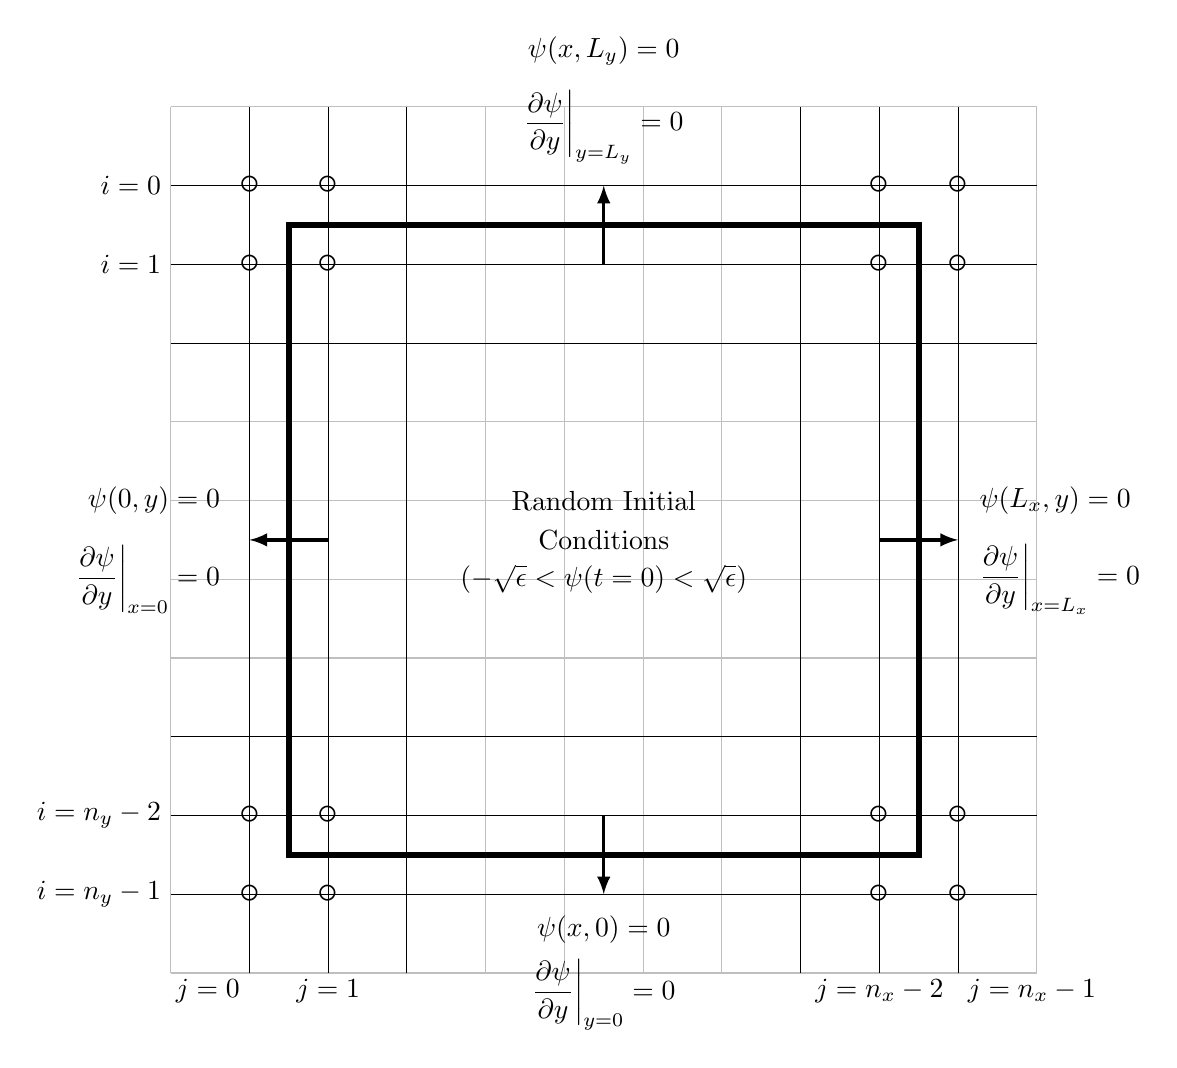
\begin{tikzpicture}
%    \fill [green!50!black,opacity=0.3] (0,10) rectangle +(5,5);
%    \fill [orange!60!black,opacity=0.3] (7,2) rectangle +(6,6);
    \draw [lightgray, thin, step = 1] (0,0) grid +(11,11);
%    \draw [black, thick, step = 5, shift = {(2.5,2.5)}];
    \draw [black, thin, step = 7, shift = {(2,2)}] (0,0) grid +(7,7);
    \draw [black, thin, step = 1, shift = {(0.,0.)}] (2,2) grid +(0,-2);
    \draw [black, thin, step = 1, shift = {(0.,0.)}] (2,2) grid +(-2,0);
    \draw [black, thin, step = 1, shift = {(0.,0.)}] (9,2) grid +(0,-2);
    \draw [black, thin, step = 1, shift = {(0.,0.)}] (9,2) grid +(2,0);
    \draw [black, thin, step = 1, shift = {(0.,0.)}] (9,9) grid +(0,2);
    \draw [black, thin, step = 1, shift = {(0.,0.)}] (9,9) grid +(2,0);
    \draw [black, thin, step = 1, shift = {(0.,0.)}] (2,9) grid +(0,2);
    \draw [black, thin, step = 1, shift = {(0.,0.)}] (2,9) grid +(-2,0);
%    \draw [black, line width=0.75mm, step = 8, shift = {(1.5,1.5)}] (0,0) grid +(8,8);
    \draw [black, thin, step = 1, shift = {(0.,0.)}] (1,1) grid +(0,-1);
    \draw [black, thin, step = 1, shift = {(0.,0.)}] (1,1) grid +(-1,0);
    \draw [black, thin, step = 1, shift = {(0.,0.)}] (10,1) grid +(0,-1);
    \draw [black, thin, step = 1, shift = {(0.,0.)}] (10,1) grid +(1,0);
    \draw [black, thin, step = 1, shift = {(0.,0.)}] (10,10) grid +(0,1);
    \draw [black, thin, step = 1, shift = {(0.,0.)}] (10,10) grid +(1,0);
    \draw [black, thin, step = 1, shift = {(0.,0.)}] (1,10) grid +(0,1);
    \draw [black, thin, step = 1, shift = {(0.,0.)}] (1,10) grid +(-1,0);
    \draw [black, thin, step = 9, shift = {(1,1)}] (0,0) grid +(9,9);
    \draw [black, thin, step = 1, shift = {(1,1)}] (2,-1) grid +(0,11);
    \draw [black, thin, step = 1, shift = {(1,1)}] (7,-1) grid +(0,11);
    \draw [black, thin, step = 1, shift = {(1,1)}] (-1,7) grid +(11,0);
    \draw [black, thin, step = 1, shift = {(1,1)}] (-1,2) grid +(11,0);
    %\draw [black] (1.5,1.5) rectangle (9.5,1.5)
	\draw[black,line width=.75mm] (1.5,1.5) rectangle (9.5,9.5);
	
	\draw [very thick,-latex] (5.5,2) -- (5.5,1);
	\draw [very thick,-latex] (2,5.5) -- (1,5.5);
	\draw [very thick,-latex] (9,5.5) -- (10,5.5);
	\draw [very thick,-latex] (5.5,9) -- (5.5,10);
	
	\node at (5.5,6) [] {Random Initial};
	\node at (5.5,5.5) [] {Conditions};   
	\node at (5.5,5) [] {$\left(-\sqrt{\epsilon}<\psi(t=0)<\sqrt{\epsilon}\right)$}; 
	
	\node at (5.5,0.85) [below] {$\psi(x,0)=0$};
	\node at (5.5,0.3) [below] {$\dfrac{\partial\psi}{\partial y}\bigg\rvert_{y=0}=0$};
	\node at (0.75,6.) [left] {$\psi(0,y)=0$};
	\node at (0.75,5.) [left] {$\dfrac{\partial\psi}{\partial y}\bigg\rvert_{x=0}=0$};
	\node at (10.15,6.) [right] {$\psi(L_x,y)=0$};
	\node at (10.15,5.0) [right] {$\dfrac{\partial\psi}{\partial y}\bigg\rvert_{x=L_x}=0$};
	\node at (5.5,11.4) [above] {$\psi(x,L_y)=0$};
	\node at (5.5,10.15) [above] {$\dfrac{\partial\psi}{\partial y}\bigg\rvert_{y=L_y}=0$};
	
	\node[scale=1.5] at (1,1) {$\circ$};
	\node[scale=1.5] at (2,1) {$\circ$};
	\node[scale=1.5] at (1,2) {$\circ$};
	\node[scale=1.5] at (2,2) {$\circ$};
	
	\node[scale=1.5] at (10,1) {$\circ$};
	\node[scale=1.5] at (9,1) {$\circ$};
	\node[scale=1.5] at (9,2) {$\circ$};
	\node[scale=1.5] at (10,2) {$\circ$};
	
	\node[scale=1.5] at (1,10) {$\circ$};
	\node[scale=1.5] at (2,10) {$\circ$};
	\node[scale=1.5] at (2,9) {$\circ$};
	\node[scale=1.5] at (1,9) {$\circ$};
	
	\node[scale=1.5] at (10,10) {$\circ$};
	\node[scale=1.5] at (10,9) {$\circ$};
	\node[scale=1.5] at (9,10) {$\circ$};
	\node[scale=1.5] at (9,9) {$\circ$};		
	
    \node at (0,10) [left] {$i=0$};    
    \node at (0,9) [left] {$i=1$};
    \node at (0,2) [left] {$i=n_{y}-2$};
    \node at (0,1) [left] {$i=n_{y}-1$};
    \node at (10,-.5) [above right] {$j=n_{x}-1$};
    \node at (9,-.5) [above] {$j=n_{x}-2$};
    \node at (1,-.5) [above left] {$j=0$};
    \node at (2,-.5) [above] {$j=1$};
    \end{tikzpicture}
\end{document}
